\documentclass[english,notitlepage]{revtex4-1}  % defines the basic parameters of the document
%For preview: skriv i terminal: latexmk -pdf -pvc filnavn



% if you want a single-column, remove reprint

% allows special characters (including æøå)
\usepackage[utf8]{inputenc}
%\usepackage[english]{babel}

%% note that you may need to download some of these packages manually, it depends on your setup.
%% I recommend downloading TeXMaker, because it includes a large library of the most common packages.

\usepackage{physics,amssymb}  % mathematical symbols (physics imports amsmath)
\include{amsmath}
\usepackage{graphicx}         % include graphics such as plots
\usepackage{xcolor}           % set colors
\usepackage{hyperref}         % automagic cross-referencing (this is GODLIKE)
\usepackage{listings}         % display code
\usepackage[most]{tcolorbox}
\usepackage{inconsolata}
\usepackage{stmaryrd}
\usepackage{enumerate}
\usepackage{subfigure}        % imports a lot of cool and useful figure commands
\usepackage{float}
%\usepackage[section]{placeins}
\usepackage{algorithm}
\usepackage[noend]{algpseudocode}
\usepackage{subfigure}
\usepackage{tikz}
\usetikzlibrary{quantikz}
% defines the color of hyperref objects
% Blending two colors:  blue!80!black  =  80% blue and 20% black
% \hypersetup{ % this is just my personal choice, feel free to change things
%     colorlinks,
%     linkcolor={red!50!black},
%     citecolor={blue!50!black},
%     urlcolor={blue!80!black}}



\newcounter{tasknr}
\newcounter{subtasknr}[tasknr]
\renewcommand{\thetasknr}{\textbf{\arabic{tasknr}}}
\renewcommand{\thesubtasknr}{\textbf{(\alph{subtasknr})}}

\newenvironment{task}[1][\thetasknr]{\refstepcounter{tasknr}\par
\bigskip \noindent\textbf{Problem~\textbf{#1}\vspace{2em})}}
	{\par\bigskip}
\newenvironment{subtask}{\par\medskip \refstepcounter{subtasknr}
\noindent \textbf{(\alph{subtasknr})}}{\par\medskip}

\newcommand{\qed}{\hfill \ensuremath{\Box}}

\definecolor{codegreen}{rgb}{0,0.6,0}
\definecolor{codegray}{rgb}{0.5,0.5,0.5}
\definecolor{codepurple}{rgb}{0.58,0,0.82}
\definecolor{backcolour}{rgb}{0.95,0.95,0.92}

\lstdefinestyle{mystyle}{
    backgroundcolor=\color{backcolour},   
    commentstyle=\color{codegreen},
    keywordstyle=\color{magenta},
    numberstyle=\tiny\color{codegray},
    stringstyle=\color{codepurple},
    basicstyle=\ttfamily\footnotesize,
    breakatwhitespace=false,         
    breaklines=true,                 
    captionpos=b,                    
    % keepspaces=true,
    % numbers=left,
    % numbersep=5pt,
    showspaces=false,                
    showstringspaces=false,
    showtabs=false,
    tabsize=2
}
\lstset{style=mystyle}

%% Defines the style of the programming listing

%% This is actually my personal template, go ahead and change stuff if you want



%% USEFUL LINKS:
%%
%%   UiO LaTeX guides:        https://www.mn.uio.no/ifi/tjenester/it/hjelp/latex/
%%   mathematics:             https://en.wikibooks.org/wiki/LaTeX/Mathematics

%%   PHYSICS !                https://mirror.hmc.edu/ctan/macros/latex/contrib/physics/physics.pdf

%%   the basics of Tikz:       https://en.wikibooks.org/wiki/LaTeX/PGF/Tikz
%%   all the colors!:          https://en.wikibooks.org/wiki/LaTeX/Colors
%%   how to draw tables:       https://en.wikibooks.org/wiki/LaTeX/Tables
%%   code listing styles:      https://en.wikibooks.org/wiki/LaTeX/Source_Code_Listings
%%   \includegraphics          https://en.wikibooks.org/wiki/LaTeX/Importing_Graphics
%%   learn more about figures  https://en.wikibooks.org/wiki/LaTeX/Floats,_Figures_and_Captions
%%   automagic bibliography:   https://en.wikibooks.org/wiki/LaTeX/Bibliography_Management  (this one is kinda difficult the first time)
%%   REVTeX Guide:             http://www.physics.csbsju.edu/370/papers/Journal_Style_Manuals/auguide4-1.pdf
%%
%%   (this document is of class "revtex4-1", the REVTeX Guide explains how the class works)


%% CREATING THE .pdf FILE USING LINUX IN THE TERMINAL
%%
%% [terminal]$ pdflatex template.tex
%%
%% Run the command twice, always.
%% If you want to use \footnote, you need to run these commands (IN THIS SPECIFIC ORDER)
%%
%% [terminal]$ pdflatex template.tex
%% [terminal]$ bibtex template
%% [terminal]$ pdflatex template.tex
%% [terminal]$ pdflatex template.tex
%%
%% Don't ask me why; I don't know.

\begin{document}

\title{Project 2}      % self-explanatory
\author{Simon Halstensen \& Herman Brunborg}          % self-explanatory
\textsc{University of Oslo}
\date{\today}                             % self-explanatory
\noaffiliation                            % ignore this, but keep it.




\maketitle 

\url{https://github.com/sim-hal/FYS3150-Project-2}

\section*{Introduction}
    
In this artice we will mainly look at ways of scaling equations, some eigenvalue problems and unit testing.

\begin{task}

We want to show that the second-order differential equation 

\begin{equation}\label{eq:differentialequation}
    \gamma \frac{d^2 u(x)}{d x^2} = -F u(x)
\end{equation}

can be written as

\begin{equation}\label{eq:dimensionlessdifferentialequation}
    \frac{d^2 u(\hat{x})}{d \hat{x}^2} = -\lambda u(\hat{x})
\end{equation}

where $\hat{x}\equiv x/L \iff x$ is a dimensionless  variable and $\lambda=\frac{F L^2}{\gamma}$. This also means that $x = \hat{x} L$. We know that

\begin{equation*}
    \frac{du}{d\hat{x}} 
    = \frac{dx}{d\hat{x}} \frac{du}{dx} 
    = L \frac{du}{dx} 
    \iff \frac{du}{dx} 
    = \frac{1}{L} \frac{du}{d\hat{x}}
\end{equation*}

we define $v=\frac{1}{L} \frac{du}{d\hat{x}}$ and get

\begin{equation*}
    \frac{d^2 u}{d x^2}
    = \frac{d}{dx} \Big( \frac{d u}{d x} \Big)
    = \frac{d}{dx} \Big( \frac{1}{L}\frac{d u}{d \hat{x}} \Big) 
    = \frac{d}{dx} \Big( v \Big) 
    = \frac{d v}{dx}
\end{equation*}

\begin{equation*}
    = \frac{d\hat{x}}{dx} \frac{dv}{d\hat{x}}
    = \frac{1}{L} \frac{dv}{d\hat{x}}
    = \frac{1}{L} \frac{d}{d\hat{x}} \Big( \frac{1}{L}\frac{d u}{d \hat{x}}  \Big)
    = \frac{1}{L^2} \frac{d^2 u}{d\hat{x}^2} 
\end{equation*}

This means that

\begin{equation*}
    \gamma \frac{d^2 u}{d x^2} = \gamma \frac{1}{L^2} \frac{d^2 u}{d\hat{x}^2} = -F u
\end{equation*}

by moving terms we see that

\begin{equation*}
    \frac{d^2 u}{d\hat{x}^2} = -F L^2 \frac{1}{\gamma} u=-\lambda u
\end{equation*}

if we evaluate $u$ on $\hat{x}$ we see that

\begin{equation*}
    \frac{d^2 u(\hat{x})}{d\hat{x}^2} = -\lambda u(\hat{x})
\end{equation*}

\qed

\end{task}



\begin{task}

We know that $\vec{v}_i$ is a set of orthonormal basis vectors, meaning $\vec{v}_i^T\cdot \vec{v}_j = \delta_{ij}$. We also know that $\bold{U}$ is an orthonormal transformation matrix. This means that $\bold{U}^T=\bold{U}^{-1}$ and that $\bold{U} \bold{U}^T=\bold{U} \bold{U}^{-1}=I$. We want to show that transformations with $\bold{U}$ preserves orthonormality, and that the set of vectors $\vec{w}_i=\bold{U}\vec{v}_i$ is also an orthonormal set. We start b looking at $\vec{w}_i=\bold{U}\vec{v}_i$

\begin{equation*}
    \vec{w}_i = \bold{U} \vec{v}_i
\end{equation*}

we transpose this equation and get

\begin{equation*}
    \vec{w}_i^T = (\bold{U} \vec{v}_i)^T = \vec{v}_i^T \bold{U}^T
\end{equation*}

this means that

\begin{equation*}
    \vec{w}_i^T \vec{w}_j = \vec{v}_i^T \bold{U}^T \bold{U} \vec{v}_j = \vec{v}_i^T I \vec{v}_j = \vec{v}_i^T \vec{v}_j = \delta_{ij}
\end{equation*}

\qed



\end{task}

\begin{task}

    See implementation
\end{task}

\begin{task}

    See implementation
\end{task}

\begin{task}

    See implementation
\end{task}

\begin{task}


\begin{figure}[h]
    \centering
    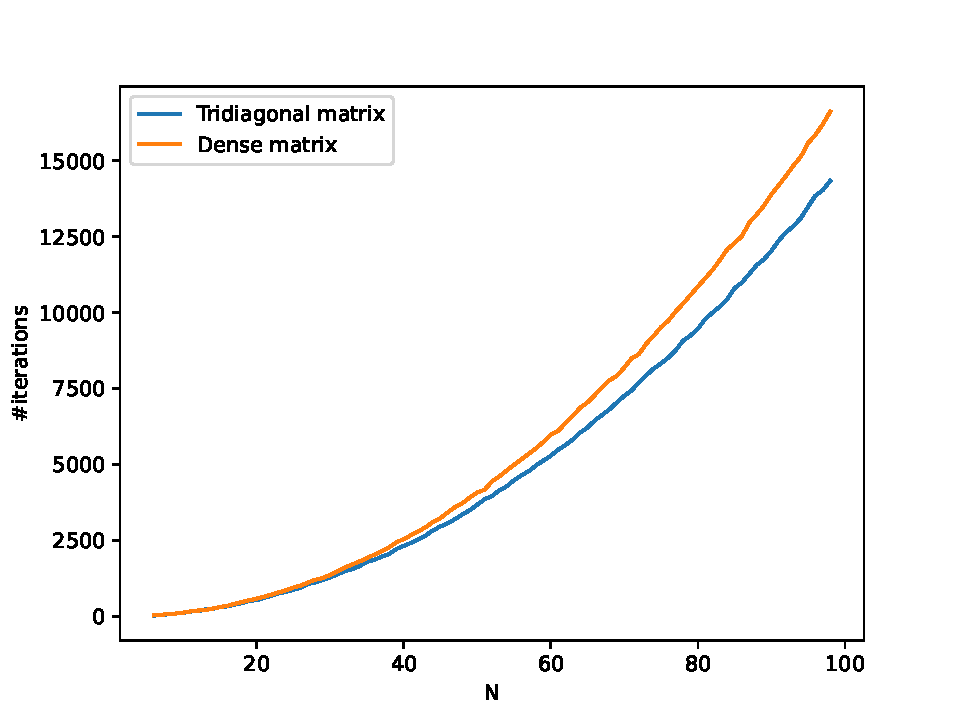
\includegraphics{output/iteration_plot.pdf}
    \caption{A plot with the number of required transformation scales}
    \label{fig:poissonplot}
\end{figure}

We suspect from reading Fig \ref{fig:poissonplot} that the scaling behavior has quadratic complexity. From the plot it seems that the dense matrix has a similar complexity, but with a somewhat bigger constant.

When we tried finding the scaling behaviour of $A$ when $A$ was a dense matrix, we saw that the size of the entries were impactful for the number of iterations. We decided to scale the matrix, so the order of magnitude of the entries was comparable to those in the tridiagonal matrix.
    
\end{task}

\end{document}
